% Compilar com: latexmk -lualatex R1.tex
\documentclass[11pt,a4paper]{article}
\usepackage[margin=2cm]{geometry}
\usepackage{fontspec}
\usepackage{unicode-math}
\setmainfont{Latin Modern Roman}
\setmathfont{Latin Modern Math}
\usepackage[brazil]{babel}
\usepackage{booktabs,array,graphicx}
\usepackage{enumitem}
\usepackage{xurl}
\usepackage[colorlinks=true,linkcolor=blue!50!black,urlcolor=blue!50!black]{hyperref}
\setlength{\parindent}{0pt}
\setlength{\parskip}{0.5em}
\newcommand{\arq}[1]{\texttt{\nolinkurl{#1}}}

\title{Fatia R1 --- parte ímpar em $\eta$ do sistemático do PHOBOS\\\large teste de simetria $\eta\leftrightarrow-\eta$ em $dN/d\eta$, Au+Au 200 GeV}
\date{17 de novembro de 2026}
\author{}

\begin{document}
\maketitle
\vspace{-2em}

\section*{Método}
Em Au+Au a física é simétrica em $\eta$. Para cada classe $c$ (11) e par $j$ ($|\eta|=0{,}1,\dots,5{,}3$; 27 pares):
\[
A_{cj}=\frac{y(\eta_j)-y(-\eta_j)}{y(\eta_j)+y(-\eta_j)}
\]
é a parte ímpar do sistemático (mais ruído). Dados: os 11 arquivos do PHOBOS usados na calibração
(\arq{HIC_experimental_data/Au-Au-200/PHOBOS}). Regiões: Octagon $|\eta|<3{,}2$ (16 pares), Rings $|\eta|>3{,}2$ (11 pares).
Script: \arq{R1_simetria_phobos.py}; resultados: \arq{R1_results.json}.

\begin{figure}[h]
\centering
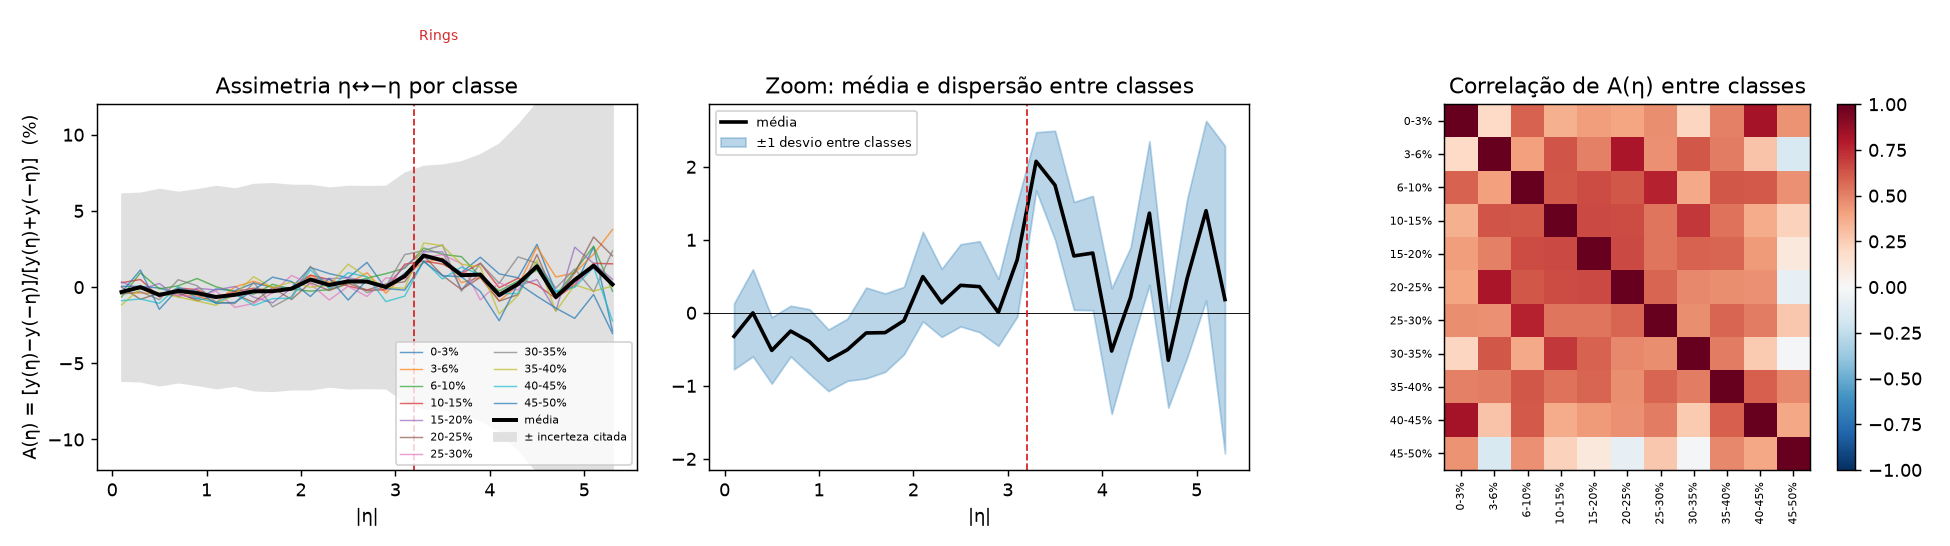
\includegraphics[width=\linewidth]{R1_simetria.png}
\caption{Esquerda: $A(\eta)$ por classe e incerteza citada (cinza). Centro: média e dispersão entre classes; linha vermelha = fronteira Octagon/Rings.
Direita: correlação de $A(\eta)$ entre classes.}
\end{figure}

\section*{Resultados}
\begin{center}
\begin{tabular}{lccc}
\toprule
região & rms de $A$ & incerteza citada & razão \\
\midrule
Octagon ($|\eta|<3{,}2$) & 0,66\% & 6,6\% & 0,10 \\
Rings ($|\eta|>3{,}2$) & 1,51\% & 11,2\% & 0,14 \\
total & 1,09\% & 8,4\% & 0,13 \\
\bottomrule
\end{tabular}
\end{center}

\begin{itemize}[nosep]
\item \textbf{Modo comum:} o primeiro modo da decomposição SVD da matriz $A$ ($11\times27$) explica 53\% da variância, com amplitude quase
igual em todas as classes (exceto 45--50\%). Correlação média de $A(\eta)$ entre classes: 0,47.
\item \textbf{Forma:} no Octagon, uma tendência suave e pequena ($-0{,}5\%$ em $|\eta|\lesssim1{,}5$ a $+0{,}4\%$ em $|\eta|\approx2$--3).
Na fronteira com os Rings, um \textbf{degrau de $\approx+2\%$} comum a todas as classes; nos Rings, um padrão alternado de
$\pm1{,}5\%$ entre bins vizinhos, também comum às classes --- compatível com a segmentação discreta dos anéis.
\end{itemize}

\section*{Leitura}
\begin{enumerate}
\item \textbf{A fonte existe e tem forma definida.} A parte ímpar é estruturada (degrau na fronteira Octagon/Rings, padrão dos anéis)
e comum às classes de centralidade: é sistemático de detector, não ruído. Isso dá, \emph{a partir dos dados}, a direção $\hat v_{\mathrm{ímpar}}$
e a escala ($\sim$0,7\% no Octagon, $\sim$1,5\% nos Rings) de uma fonte do modelo $\sum_a\lambda_a\hat v_a$.
\item \textbf{É pequena frente à incerteza total}: 10--14\% da incerteza citada. A maior parte do sistemático do PHOBOS é par em $\eta$
(normalização --- fatia 2a --- e forma par --- R3--R5).
\item \textbf{3º momento: não mensurável aqui.} A assimetria dos valores de $A$ ($+0{,}46\pm0{,}17$) descreve a \emph{forma do perfil em $\eta$},
não a distribuição de probabilidade da fonte: há essencialmente \emph{uma} realização (uma análise do PHOBOS) vista em muitos $\eta$, com as
classes fortemente correlacionadas. A assimetria das amplitudes do modo 1 ($-1{,}8$, $N=11$) é dominada por uma única classe (45--50\%).
Para o 3º momento seriam necessárias muitas realizações independentes da fonte.
\end{enumerate}

\section*{Ressalvas}
\begin{itemize}[nosep]
\item Supõe-se que efeitos de vértice e aceitação foram corrigidos na publicação; um resíduo deles apareceria como parte ímpar.
\item O padrão alternado nos Rings pode também refletir a binagem/interpolação usada para gerar os arquivos da calibração; verificar contra a tabela original.
\item Só a parte ímpar é vista; a parte par da fonte por região exige R3--R5.
\end{itemize}
\end{document}
